\section{Performing validation with Geant-val}
\label{sec-workflow}

Geant4 validation procedure consists of two big steps: generating results (executing the tests and importing their output into Geant-val) and analysing these results.

\section{Generating results}

\subsection{Running the tests}

To manage a set of Geant4 tests and their configurations, a {\tt mc-config-generator} Python framework was developed. It allows one to configure and run test jobs in various batch systems (CERN LSF, HTCondor, Torque PBS), and to convert the results into  JSON format for further uploading to the application database. The framework is not Geant4-specific, and can be used with other projects (e.g., Pythia8). Source code is available in corresponding Git repository\footnote{https://gitlab.cern.ch/GeantValidation/geant-config-generator}.

Each test supported by the {\tt mc-config-generator} consists of a "parameters" file, containing all combinations of parameters used by the given test, and one or more "template" files.

\subsection{Importing test results into Geant-val}

We use JSON, like shown in Appendix~\ref{adx:JSON-format}, for importing data into the database and for exchanging information between different parts of the web application. Each JSON file contains one plot scatter plot or 1D histogram, along with additional data:

\begin{itemize}
    \item Name of the measured physics value (\textit{observable}), which used for matching \textit{plot} to the experimental data (e.g., differential cross-section);
    \item The name and version of tool (e.g., Geant4 and 10.5.beta01);
    \item Name of the test (e.g. Tileatlas);
    \item Name(s) and value(s) of the parameters used for running the test (e.g. Physics List: FTFP\_BERT);
    \item For experimental data, Inspire~\cite{inspire} or HepDATA~\cite{hepdata} ID of the original article.
\end{itemize}

For the supported tests, the parser script in {\tt mc-config-generator} framework can be used to convert text and/or ROOT files produced by the test into JSON format. The conversion is done in multiple threads to minimise the execution time.

Geant4 developers can upload JSON files by sending a HTTP POST request to \textsf{Geant-val} website using {\tt geant\_upload.py}\footnote{https://gitlab.cern.ch/GeantValidation/GVP/raw/master/scripts/geant\_upload.py} command-line utility.

After uploading the results, these are available on the website for further analysis.

\section{Analysing data}
\label{sec-analyse}

The \textsf{Geant-val} website provides two ways of viewing and comparing results:

\begin{figure}[h]
    \centering
    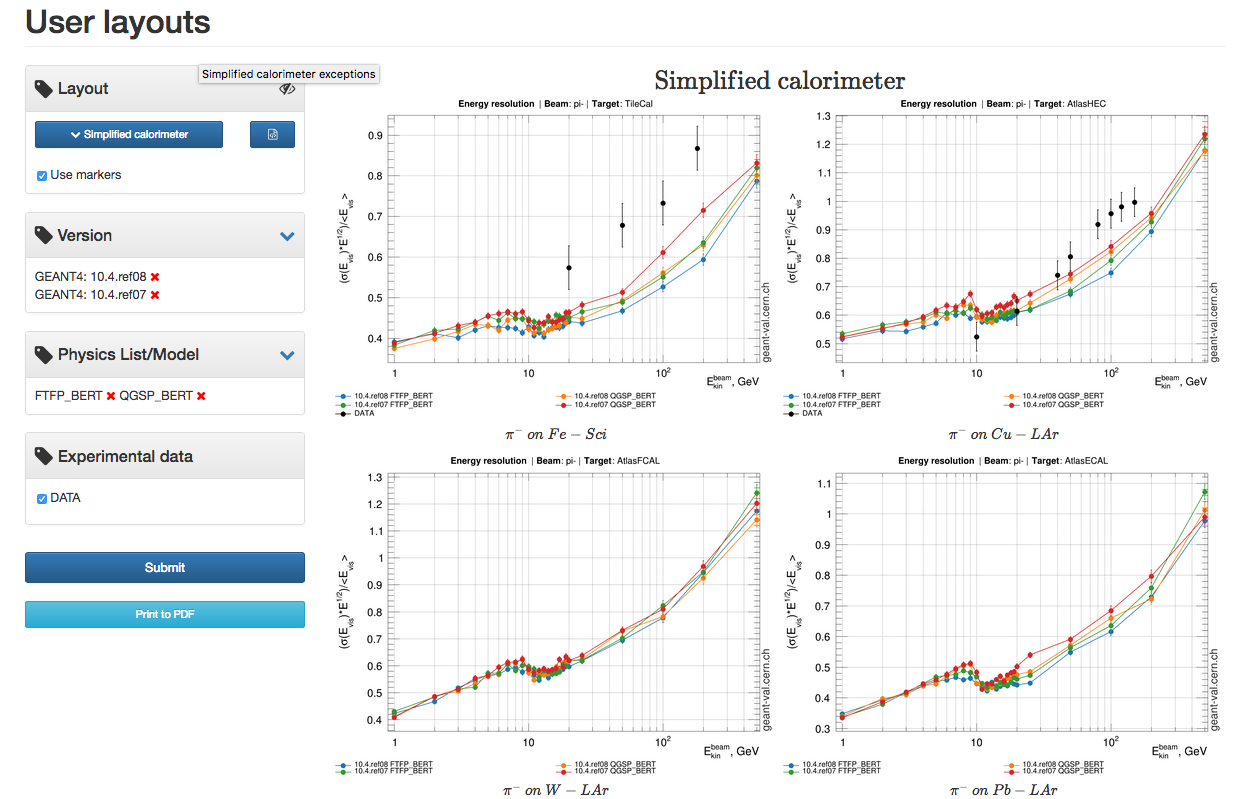
\includegraphics[width=0.8\textwidth,clip]{layout_sc.png}
    \caption{Example of user defined layout for the Geant4 "simplified calorimeter" test showing test results for two Geant4 reference releases - 10.4.ref07 and 10.4.ref08.}
    \label{fig:layouts}
\end{figure}

\textit{Statistical comparisons} page (see Fig.~\ref{fig:statcomparison}) allows one to perform comparison of simulation with compatible experimental results using statistical tests. % It displays results of statistical comparison for pairs of plots with the same parameters' values.
Currently $\chi^2$ ($\chi^2/n.d.f.$, $\chi^2$ probability) and Kolmogorov-Smirnov (KS Max(D), KS probability) tests are implemented. All computations are performed asynchronously on the client side using JavaScript WebWorkers. For this purpose, JavaScript code to perform $\chi^2$ and Kolmogorov-Smirnov tests have been written, and their results cross-checked against the same statistical techniques implemented in the ROOT framework.

\begin{figure}[h]
    \centering
    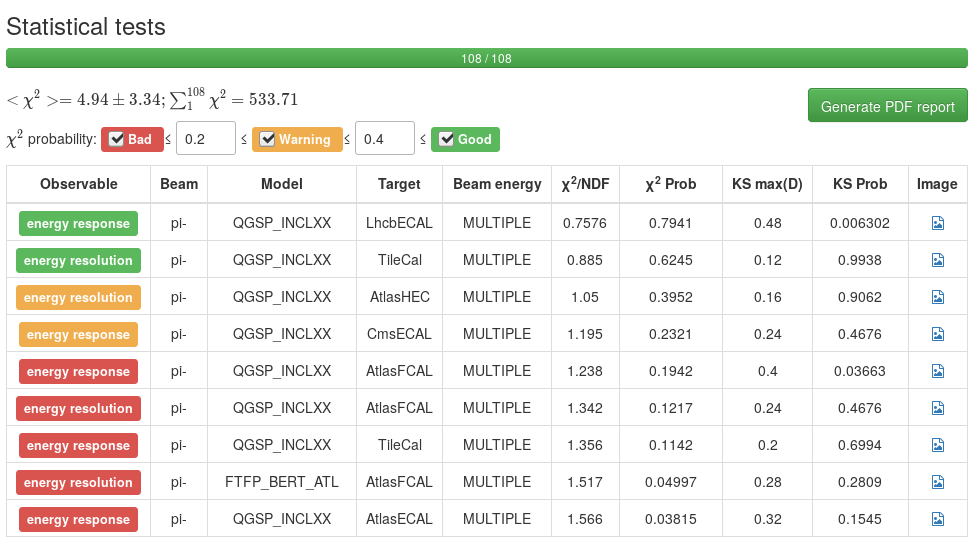
\includegraphics[width=0.8\textwidth,clip]{statcomparison.png}
    \caption{Example of statistical comparison between two official Geant4 releases, 10.5.beta01 and 10.4.p02, for the "simplified calorimeter" test.}
    \label{fig:statcomparison}
\end{figure}

\textit{User layouts} page (see Fig.~\ref{fig:layouts}). Some Geant4 tests produce hundreds of different plots, but for fast "visual" validation it is often enough to compare only a small well-defined subset of them. The \textit{User layout} is an XML file describing what plots should be displayed and how should they be laid out on a page. User can use one of the existing layouts or define their own one (see Appendix~\ref{adx:XML-format}).
